
% Introduction
During the spread of an epidemic, numerous surveillance systems collect data about infected cases \cite{Thomas et al 2015}. These include notifications of confirmed cases from health care providers, voluntary surveys, internet search queries, and many more \cite{}. Different sources of data tend to capture different aspects of disease transmission, from the onset of symptoms, confirmation of positive cases, and outcomes of the disease (i.e. recovery or fatality) \cite{Moss et al 2016}.
By combining observed data with mathematical models, it is possible to estimate model parameters, forecast the spread of the epidemic, and inform public health decision-making \cite{Keeling Rohani 2007, Held 2020}.
It is often desirable to estimate model parameters as more data become available. Bayesian statistics provides the natural framework for updating parameter estimates as more data become available \cite{Spiegelhalter 2019}. These estimates can then be utilised to enable the calculation of key epidemiological quantities and the evaluation of public health intervention measures, such as vaccination programmes. However, most approaches only consider one source of data \cite{Ross et al 2010}.
In this paper, we propose a model for seasonal influenza that integrates multiple sources of data simultaneously, and present an approach for estimating the model's parameters using the Metropolis-Hastings algorithm.
This paper is structured in the following way. Section 2 provides a full description of the epidemic model and the Bayesian inference framework, including a derivation of the likelihood and the implementation of the Metropolis-Hastings algorithm. Section 3 contains an implementation of the epidemic simulation and the results from the parameter estimation. Finally, section 4 contains a discussion of the methods and results, including potential directions for future work.

\section{Sources of Data} 
Many surveillance systems are used to collect data during the influenza season each year, usually from April/May to October. These systems may record data on different timescales, for example in real-time, or at daily, or weekly intervals. They may also capture different aspects of the underlying epidemic, from the onset of symptoms to hospital admissions \cite{Thomas et al 2015, Moss et al 2016}. Some of the more common surveillance systems are discussed below.

\subsection{Case Notifications}
In Australia, laboratory-confirmed influenza is a `notifiable' disease \cite{Dep of Health 2020}. That is, when a person presents to a health service such as a general practitioner (GP) or hospital with influenza-like symptoms, a sample may be taken from the patient's respiratory tract and sent to a laboratory for testing. If the test returns a positive result for influenza, a notification is sent to the local state or territory health authority. These case notifications ($C$) are then sent to the Australian Department of Health, where they are collected in the National Notifiable Disease Surveillance System.\\
Notification data are given unique reference numbers, and include information about the state or territory, disease code, date of onset and notification, gender, age, indigenous status, and the patient's postcode.
Case notification data are collected all year round and freely available on the Department of Health website. However, delays between the onset of symptoms, seeking medical care, and processing time in the laboratory lead to delays in the data \cite{Clothier 2006}. Another limitation of case notifications is that data are only collected for cases that are severe enough to warrant seeking medical attention, and may skew the data towards over representing groups at risk, for example the elderly.

\subsection{FluCAN}
The Influenza Complications Alert Network (FluCAN or $FC$) is a hospital-based surveillance network that consists of 17 hospitals across all states and territories in Australia. FluCAN collects data on patients who are admitted to one of these hospitals suffering from acute respiratory illness with influenza later confirmed by laboratory analysis. Demographic information collected in FluCAN includes the patient's age, Aboriginal or Torres Strait Islander status, health risk factors and vaccination status. Clinical information collected includes length of hospital stay, admission to intensive care, and case fatality. FluCAN data is used in statistical analysis to estimate quantities such as national influenza hospital admission and vaccine effectiveness.
The objective of FluCAN is to collect information about patients admitted to hospital with influenza in order to help inform public health policy \cite{Cheng 2017}.
During the 2016 flu season, 1952 patients with laboratory-confirmed influenza were recorded in FluCAN.

\subsection{FluTracking}
FluTracking ($FT$) is an online surveillance system that relies on volunteers to register by email and then complete short online surveys each week during flu season \cite{Moss et al 2019}.
Participants are initially asked to provide non-identifying information such as year of birth, gender, and postcode.
Survey questions ask whether the participant had displayed any influenza-like symptoms, sought medical treatment, or been tested for an influenza-like-illness ($ILI$) over the previous seven days. Participants' vaccination status for that year is also collected. Surveys typically take under 15 seconds to complete. An example of a survey from a week in September 2020 is given in Figure \ref{fig:FluTracking Survey}.
The goal of FluTracking is to provide community-level surveillance of ILI, in particular influenza, and more recently COVID-19. This data is then used to generate regular reports, and analysed to give insight into the geographic and demographic distribution of ILI in the community. The advantage of FluTracking is that it collects information about symptomatic cases that may not present to health services such as general practitioners and hospitals.
In 2019 over 50,000 participants in Australia answered at least one weekly survey.

\begin{figure}[h!]
	\centering
	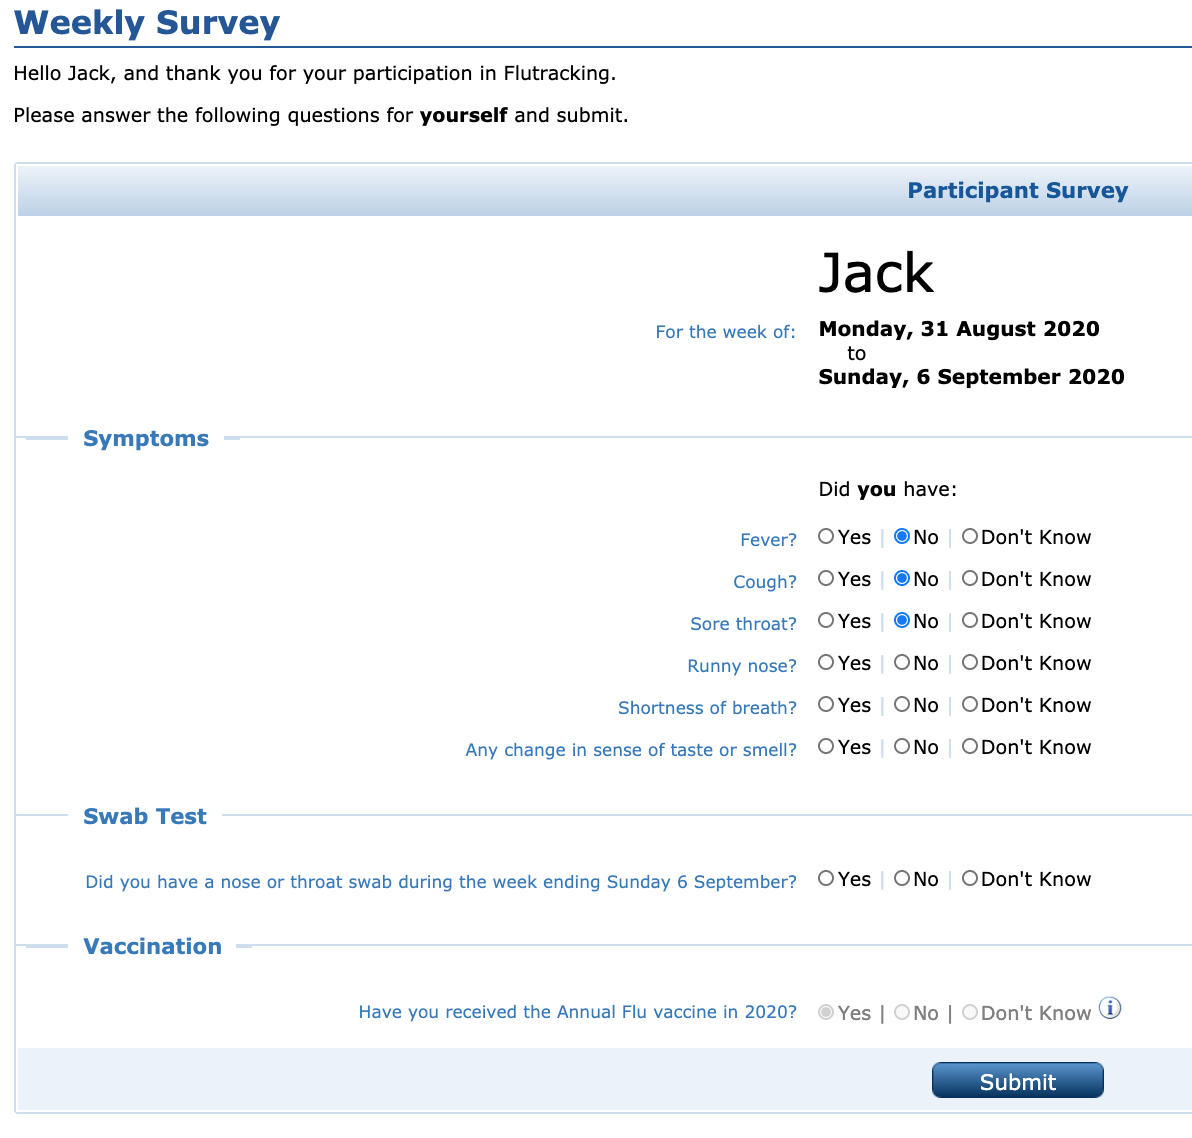
\includegraphics[scale=0.5]{Figs/FluTrackingSurvey.png}
	%		\vspace{-10mm}
	\caption{An example FluTracking survey for a week in September 2020. Participants are asked about the presence of ILI symptoms, if they have been tested for influenza, and if they have been vaccinated this season. If any of these questions are responded to in the positive the participant is prompted to answer further questions such as whether they contacted a health professional, whether they were tested, and if so the result of the test.}
	\label{fig:FluTracking Survey}
\end{figure}

\subsection{First Few Hundred Studies}
A First Few Hundred (FF100) study is a surveillance activity undertaken during the initial stages of an epidemic on the first few hundred laboratory-confirmed cases \cite{Mclean et al 2010}.
Data are collected from households with a confirmed case either in person or by telephone at two points in time; soon after the positive laboratory-confirmed result, and again fourteen days later.
The data comprise demographic information (e.g. age, sex, occupation), and clinical information such as types of symptoms, date of symptom onset, severity of disease, any medical conditions or co-morbidities, and vaccination status.
Details about contact with others either within or outside the household are also obtained, and these contacts are also interviewed. Contacts who subsequently become symptomatic and test positive then become cases themselves.
The purpose of the 14-day follow up is to determine the duration of illness, the outcome (e.g. death/recovery), as well as the occurrence of any treatments or complications.
FF100 studies enable the early assessment of an epidemic, particularly of novel strains that have the potential to become pandemic, in order to allow epidemiological forecasting and inform public health decision making.
\\ \\
The four sources of data presented here were originally included in the epidemic model constructed by the MATRIX group. In this project, FF100 data are not considered in order to keep the model relatively simple (this is discussed later).
However there are many other sources of data that could be included in a multi-data epidemic model which are not considered here such as Google Flu Trends and smartphone contact tracing apps.

\subsection{Recent Research (integrate into Intro)}
Over the last ten years much work has been done on household epidemic models, including the development of efficient computational methods, using MCMC methods for estimating model parameters \cite{Ross et al 2010, Black Ross 2013, Geard et al 2013, Black et al 2013, Black Ross 2013, Ristic Dawson 2013, Walker et al 2017}.
Most of this research has focussed on a single source of data. Moss \textit{et al.} used weekly FluTracking data to estimate the probability that a person with an ILI would go to a GP and give a sample to be tested \cite{Moss et al 2019}. These estimates were then incorporated into weekly forecasts of seasonal influenza during 2017 and were found to have improved the predictive accuracy of the forecasts. Walker \textit{et al.} (2017) introduced and compared two novel methods for inferring transmission parameters for a stochastic household epidemic model using information provided by a FF100 data set \cite{Walker et al 2017}. Black \textit{et al.} presented a method for analysing data from a FF100 study in order to obtain an early assessment of the severity and transmissibility of pandemic influenza \cite{Black et al 2017}. Zarebski \textit{et al.} present a method for choosing an optimal model for forecasting seasonal influenza cases using laboratory-confirmed case notification data  \cite{Zarebski et al 2017}.\\
More recently, studies have emerged that consider multiple sources of data.
Moss \textit{et al}. (2016) attempted to evaluate epidemic forecasts using three sources of data: Google Flu Trends, clinical observations, and laboratory-confirmed case notifications \cite{Moss et al 2016}.
Initially, results were obtained using each source of data individually. It was found that in each case the timing of the peak of the epidemic could be forecast accurately four-six weeks in advance. Then, all three sources of data were combined into a single data set and it was attempted to determine if utilising multiple sources of data improved predictive skill. Moss \textit{et al.} concluded that taking into account just two sources of data still presents a fundamental challenge to improving forecasting accuracy.\\
A collaboration between the university of Melbourne and the Defence Science and Technology Group may have successfully integrated multiple data sources with the development of two epidemic modelling tools, EpiDefend and EpiFX \cite{McCaw et al 2018}. EpiDefend is an epidemic detection tool that is reported to combine data from confirmed cases of influenza, anonymised GP reports, and other environmental data such as humidity. Weekly forecasts provide a measure of background ILI incidence and enable the detection of spikes that could indicate either epidemic outbreak or bioterrorism attack. EpiFX is a forecasting tool that combines surveillance data such as hospital admissions and social media posts to produce weekly forecasts. Both tools have the potential to be used for other notifiable diseases and are applicable to both public health and national defence, such as detecting bioterrorism attacks domestically or in an operational environment. No peer-reviewed publications of this work could be found, however both tools are purportedly being used by the Victorian Health Department.\\
Despite the recent research on household epidemic models and the use of MCMC methods, a Bayesian framework for utilising multiple sources of data simultaneously remains elusive. The purpose of this project is to provide a proof of concept for an efficient, accurate Bayesian framework that integrates multiple sources of data. The following chapters provide a description of an epidemic model that integrates FluTracking, FluCAN and case notification data sets, the design and implementation of the Bayesian inference methods, and the results of an attempt to estimate the model parameters using synthetically generated data.


% One of the tools used to inform public health decision making is mathematical modelling \cite{Held 2020}.
% Modelling the spread of an infectious disease can provide two types of information: qualitative insights into the dynamics of the disease, such as conditions that determine whether or not an epidemic outbreak will occur; and quantitative information, such as forecasts of the number of people who will be infected, or the duration of the epidemic \cite{Keeling Rohani 2007}. In order to produce this information, mathematical models require data.
% Numerous surveillance systems generate data at regular intervals during the spread of an epidemic \cite{Thomas et al 2015}. These include notifications of confirmed influenza cases from health care providers, health surveys, internet search queries, and many more. Different sources of data tend to capture different aspects of the underlying epidemic \cite{Moss et al 2016}.
% It is often desirable to use the data as they become available. By combining mathematical models and observed data, Bayesian statistics provides the natural framework for updating estimates of key quantities, such as model parameters, as more data become available \cite{Spiegelhalter 2019}. These estimates can then enable the calculation of other key epidemiological quantities and the evaluation of public health intervention measures such as physical distancing and vaccination programmes. However, most approaches only consider one source of data \cite{Ross et al 2010}. Recently, interest has grown in models that integrate more than one source of data \cite{Moss et al 2016}.
% Three goals: (i) to provide a complete description of the multi-data household epidemic model, (ii) to implement the model using efficient computational methods, and (iii) to develop a framework for Bayesian inference that produces an accurate estimation of the model's parameters.